\section[PLANO MACRO DO PROCESSO DE MONTAGEM (ENTREGA 3)]{PLANO MACRO DO PROCESSO DE MONTAGEM\\(ENTREGA~3)}
\label{sec:plano_macro}

O planejamento do processo tem dois níveis. O plano macro fornece a sequência de operações, as máquinas e os equipamentos e os tempos, e é usado pelo planejamento e controle da produção para programar a fabricação ou a montagem. O detalhamento das operações produz as instruções colocadas ao lado do posto de trabalho e garante a repetibilidade de cada operação \cite{rozenfeld2006gestao}. Esta seção trata do primeiro nível para a montagem do Tag\&Go.

O plano cobre a montagem do dispositivo preso à peça de roupa, com a mesma fronteira da estrutura do produto. A fabricação das peças, a base de recarga, o servidor e as páginas de cadastro e de compra ficam fora. O ponto de partida é a sequência da versão aprimorada pelo DFMA (Tabela~\ref{tab:dfma_tempos_aprimorado}), que já segue a montagem de baixo para cima da vista em camadas (Figura~\ref{fig:conj_camadas}).

% ---------------------------------------------------------------------
\subsection{Premissas}
\label{subsec:plano_premissas}

O plano adota cinco premissas.

\begin{itemize}
  \item \textbf{Versão do produto.} O plano monta a versão aprimorada, com as mudanças M1 a M8 (Tabela~\ref{tab:dfma_mudancas}). Como M7 e M8 ainda não foram avaliadas, a Subseção~\ref{subsec:plano_pendencias} registra o que muda sem elas.

  \item \textbf{Produto de série.} O plano descreve a montagem do produto, e não a do protótipo. O protótipo usa componentes de mercado sem solda, em uma caixa de 210~$\times$~76~$\times$~54~mm (Subseção~\ref{subsec:conj_prototipo}), e sua montagem serve para conferir a ordem das operações, não os tempos.

  \item \textbf{Montagem manual em célula.} A primeira implantação está limitada a uma loja (Subseção~\ref{subsec:comerc_cobertura}), e esse volume não justifica linha automatizada nem posto dedicado por operação. A montagem é feita em uma célula de bancadas, com um operador que percorre os postos na ordem do fluxo.

  \item \textbf{Peças recebidas prontas.} As peças fabricadas chegam dos fornecedores já moldadas, fundidas ou usinadas, pelos processos da Subseção~\ref{subsec:plano_processos}. Os itens comprados montados, como a embreagem, o microatuador e a placa de controle, chegam prontos, e o firmware da placa é gravado pelo fornecedor dela. A gravação do código 2D na tampa é feita pela equipe, porque o endereço de cada dispositivo precisa ser registrado no servidor.

  \item \textbf{Tempos.} Os tempos das operações de montagem são os da análise DFA, estimados por classe de dificuldade \cite{boothroyd2011product}. A inspeção, a gravação do código, a cura, o teste e a embalagem não têm tempo de referência nessas tabelas e serão cronometradas no protótipo.
\end{itemize}

% ---------------------------------------------------------------------
\subsection{Processos de fabricação das peças}
\label{subsec:plano_processos}

As seis peças fabricadas sob desenho chegam prontas à célula. A Tabela~\ref{tab:plano_processos} registra o processo de cada uma, escolhido pelos atributos de volume, complexidade da forma, precisão e custo \cite{rozenfeld2006gestao}, e o processo equivalente no protótipo.

\begin{table}[htbp]
    \centering
    \caption{Processos de fabricação das peças fabricadas}
    \label{tab:plano_processos}
    \footnotesize
    \renewcommand{\arraystretch}{1.3}
    \begin{tabularx}{\textwidth}{@{}
        >{\RaggedRight\arraybackslash}p{2.6cm}
        >{\RaggedRight\arraybackslash}p{2.5cm}
        >{\RaggedRight\arraybackslash}X
        >{\RaggedRight\arraybackslash}p{3.2cm}@{}}
        \toprule
        \textbf{Peça} & \textbf{Material} & \textbf{Processo e máquina na série} & \textbf{Protótipo} \\
        \midrule
        Base (TG-111) & PC/ABS & Moldagem por injeção, em injetora com molde de duas placas & Impressão 3D em PLA \\
        Tampa (TG-112) & PC/ABS para laser & Moldagem por injeção. O código 2D é gravado depois, no Posto 0 & Impressão 3D em PLA, com o código colado \\
        Suporte (TG-113) & POM copolímero & Moldagem por injeção, com o ponto de injeção perto da prateleira & Impressão 3D em PLA \\
        Garra (TG-211) & Al 6061-T6 & Usinagem em centro de usinagem CNC nos lotes pequenos. Com a M2, fundição sob pressão em liga de fundição & Impressão 3D em PLA \\
        Braço dos ímãs (TG-312) & Al 6061-T6 & Usinagem em centro de usinagem CNC, em uma só fixação & Impressão 3D em PLA \\
        Guia de luz (TG-412) & PC transparente & Moldagem por injeção & Não se aplica \\
        \bottomrule
    \end{tabularx}
    \source{Elaborado pelos autores (2026).}
\end{table}

Na primeira implantação, limitada a uma loja, o volume não paga os moldes de injeção e de fundição. Até a frota crescer, as peças plásticas podem ser usinadas ou impressas em material de engenharia, com as mesmas cotas.

% ---------------------------------------------------------------------
\subsection{Organização da montagem}
\label{subsec:plano_organizacao}

A montagem foi dividida em seis postos (Figura~\ref{fig:plano_fluxo}). O Posto 0 prepara as peças por lote, fora do fluxo unitário. Os Postos 1 e 2 montam os subconjuntos do mecanismo e da tampa, que podem ser feitos em paralelo. O Posto 3 faz a montagem final, o Posto 4 testa e cadastra o dispositivo, e o Posto 5 o prepara para a expedição.

\begin{figure}[htbp]
\centering
\caption{Fluxo da montagem do Tag\&Go por posto}
\label{fig:plano_fluxo}
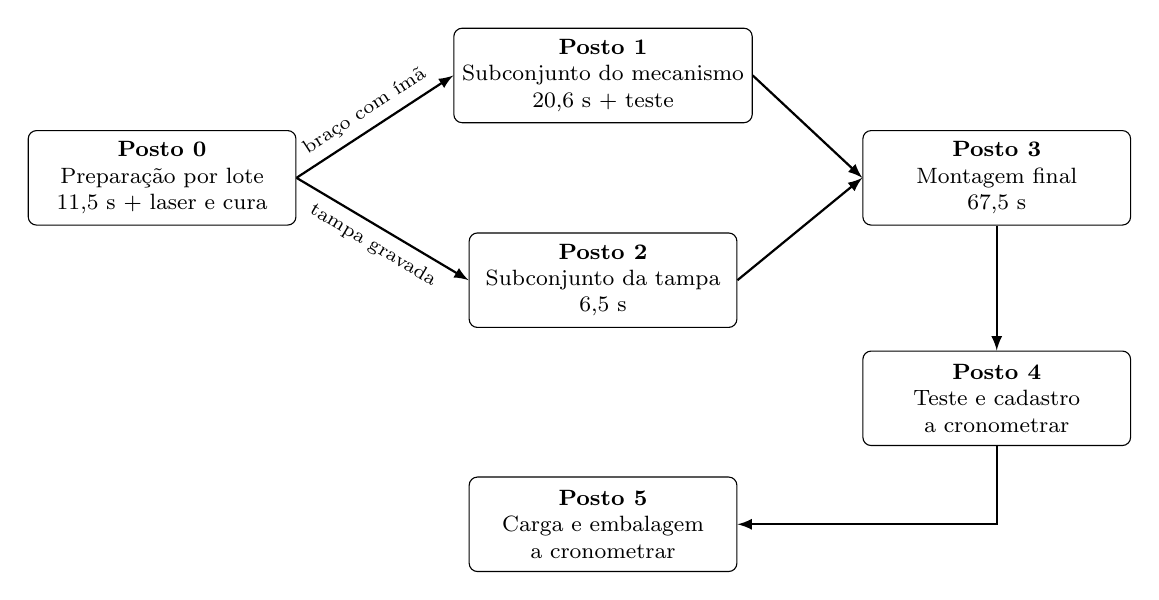
\begin{tikzpicture}[
  posto/.style={draw, rounded corners=3pt, align=center, font=\footnotesize,
                minimum width=3.4cm, minimum height=1.2cm, inner sep=3pt},
  seta/.style={-latex, thick}]
  \node[posto] (p0) at (0,0)    {\textbf{Posto 0}\\Preparação por lote\\11,5 s + laser e cura};
  \node[posto] (p1) at (5.6,1.3)  {\textbf{Posto 1}\\Subconjunto do mecanismo\\20,6 s + teste};
  \node[posto] (p2) at (5.6,-1.3) {\textbf{Posto 2}\\Subconjunto da tampa\\6,5 s};
  \node[posto] (p3) at (10.6,0)  {\textbf{Posto 3}\\Montagem final\\67,5 s};
  \node[posto] (p4) at (10.6,-2.8) {\textbf{Posto 4}\\Teste e cadastro\\a cronometrar};
  \node[posto] (p5) at (5.6,-4.4) {\textbf{Posto 5}\\Carga e embalagem\\a cronometrar};
  \draw[seta] (p0.east) -- node[midway, above, sloped, font=\scriptsize] {braço com ímã} (p1.west);
  \draw[seta] (p0.east) -- node[midway, below, sloped, font=\scriptsize] {tampa gravada} (p2.west);
  \draw[seta] (p1.east) -- (p3.west);
  \draw[seta] (p2.east) -- (p3.west);
  \draw[seta] (p3.south) -- (p4.north);
  \draw[seta] (p4.south) |- (p5.east);
\end{tikzpicture}
\begin{center}
Fonte: Elaborado pelos autores (2026).
\end{center}
\end{figure}

A sequência mantém a da Tabela~\ref{tab:dfma_tempos_aprimorado}, com uma exceção. Na análise DFA, o adesivo e o ímã eram aplicados com o braço já preso ao microatuador, e a cura ocorria com o subconjunto do mecanismo parado. No plano, o ímã é colado no braço no Posto 0, por lote e com um gabarito que fixa a altura do ímã no alojamento. A mudança traz três vantagens. A cura sai do fluxo unitário, a folga de 0,2~mm até a prateleira passa a ser controlada por um gabarito, e não pela mão do operador, e o Posto 1 recebe o braço pronto para a prensa. Os tempos das duas operações não mudam, apenas passam de posto. Em contrapartida, o braço chega ao Posto 1 já com o ímã, que atrai ferramentas e peças de aço. Por isso o Posto 1 usa ferramentas não magnéticas, e o tempo de manuseio do braço deve ser conferido na cronometragem.

O Posto 1 termina com um teste do subconjunto, antes que ele entre na base. É a vantagem que justificou manter o suporte separado da base na análise DFMA (Subseção~\ref{subsec:dfma_regras}): uma falha do mecanismo é encontrada antes de a carcaça ser fechada, sem desmontar a eletrônica.

% ---------------------------------------------------------------------
\subsection{Sequência de operações}
\label{subsec:plano_sequencia}

A Tabela~\ref{tab:plano_macro} apresenta o plano macro. Cada operação recebe um número no formato posto.ordem. A coluna de origem indica o número da operação na Tabela~\ref{tab:dfma_tempos_aprimorado}, de onde vem o tempo, ou indica que a operação foi acrescentada pelo plano.

{\footnotesize
\setlength{\tabcolsep}{4pt}
\renewcommand{\arraystretch}{1.2}
\begin{longtable}{@{}c >{\raggedright\arraybackslash}p{5.4cm} >{\raggedright\arraybackslash}p{4.4cm} c c@{}}
\caption{Plano macro do processo de montagem do Tag\&Go}
\label{tab:plano_macro} \\
\hline
\textbf{Nº} & \textbf{Operação} & \textbf{Máquina, equipamento ou ferramenta} & \textbf{Origem} & \textbf{Tempo (s)} \\
\hline
\endfirsthead
\multicolumn{5}{l}{\textit{Tabela~\thetable\ (continuação)}} \\
\hline
\textbf{Nº} & \textbf{Operação} & \textbf{Máquina, equipamento ou ferramenta} & \textbf{Origem} & \textbf{Tempo (s)} \\
\hline
\endhead
\hline
\multicolumn{5}{r}{\textit{continua na próxima página}} \\
\endfoot
\hline
\endlastfoot
\multicolumn{5}{l}{\textbf{Posto 0 -- Preparação (por lote)}} \\
0.1 & Inspeção de recebimento por amostragem: campo dos ímãs, tensão das células e espessura e planicidade da prateleira do suporte & Gaussímetro, multímetro e paquímetro & Plano & Por lote \\
0.2 & Gravação do código 2D na face da tampa & Máquina de marcação a laser, com gabarito de posicionamento da tampa & Plano & A cronometrar \\
0.3 & Verificação da leitura do código e registro do endereço & Leitor de código 2D e computador & Plano & A cronometrar \\
0.4 & Adesivo no alojamento do braço (TG-312) & Dosador de adesivo & 5 & 6,0 \\
0.5 & Ímã único (TG-313) no braço, com a altura fixada pelo gabarito & Gabarito de colagem e pinça não magnética & 6 & 5,5 \\
0.6 & Cura do adesivo & Estante de cura & Plano & Conforme o adesivo \\
\multicolumn{3}{r}{\textit{Subtotal do Posto 0, sem gravação e cura}} & & \textit{11,5} \\
\hline
\multicolumn{5}{l}{\textbf{Posto 1 -- Subconjunto do mecanismo}} \\
1.1 & Suporte (TG-113) no dispositivo de fixação & Dispositivo de fixação do suporte & 1 & 2,6 \\
1.2 & Embreagem (TG-222) no alojamento do suporte & Manual & 2 & 3,5 \\
1.3 & Microatuador (TG-311) no suporte, na posição de repouso & Manual & 3 & 3,8 \\
1.4 & Braço com o ímã no eixo do microatuador, por pressão (M3) & Prensa manual de bancada, com batente de altura e ferramental não magnético & 4 & 6,8 \\
1.5 & Chave da garra (TG-512) no suporte (M8) & Manual & 7 & 3,9 \\
1.6 & Teste do subconjunto: folga entre o ímã e a prateleira, giro de 90$^\circ$ com retorno e liberação de um pino-padrão & Bancada de teste do mecanismo, com fonte, controlador de teste, pino-padrão e calibre de folga não magnético & Plano & A cronometrar \\
\multicolumn{3}{r}{\textit{Subtotal do Posto 1, sem o teste}} & & \textit{20,6} \\
\hline
\multicolumn{5}{l}{\textbf{Posto 2 -- Subconjunto da tampa}} \\
2.1 & Tampa (TG-112) no dispositivo, com a face gravada para baixo & Dispositivo de fixação da tampa, com apoio que protege a gravação & 8 & 2,6 \\
2.2 & Guia de luz (TG-412) na tampa, por encaixe (M6) & Manual & 9 & 3,9 \\
\multicolumn{3}{r}{\textit{Subtotal do Posto 2}} & & \textit{6,5} \\
\hline
\multicolumn{5}{l}{\textbf{Posto 3 -- Montagem final}} \\
3.1 & Base (TG-111) no dispositivo de fixação & Dispositivo de fixação da base, em bancada antiestática & 10 & 2,6 \\
3.2 & Bobina (TG-522) no fundo da base & Manual & 11 & 4,4 \\
3.3 & Célula (TG-521) sobre a bobina & Manual, com procedimento de manuseio de célula de lítio & 12 & 3,3 \\
3.4 & Placa (TG-511), já com o LED de três cores, sobre a célula & Manual, com pulseira antiestática & 13 & 4,3 \\
3.5 & Subconjunto do mecanismo na base & Manual & 14 & 4,3 \\
3.6 & Conectores da bobina, da célula, do microatuador e da chave da garra na placa & Manual, com pulseira antiestática & 15 & 16,0 \\
3.7 & Subconjunto da tampa sobre a base, com as abas encaixadas (M4) & Manual & 16 & 4,3 \\
3.8 & Dois parafusos da tampa (TG-121), no lado do mecanismo & Parafusadeira elétrica com controle de torque e ponta não imantada & 17 & 17,0 \\
3.9 & Mola de abertura (TG-213) no alojamento da garra (M7) & Pinça; molas fornecidas separadas & 18 & 4,5 \\
3.10 & Garra fundida (TG-211) nos mancais da tampa, por encaixe (M2 e M7) & Manual & 19 & 6,8 \\
\multicolumn{3}{r}{\textit{Subtotal do Posto 3}} & & \textit{67,5} \\
\hline
\multicolumn{5}{l}{\textbf{Posto 4 -- Teste e cadastro}} \\
4.1 & Dispositivo na base de recarga: detecção da recarga pela placa (M5) e indicação de recarga & Base de recarga & Plano & A cronometrar \\
4.2 & Vínculo entre o código 2D e o identificador da placa no servidor & Leitor de código 2D e computador com o \textit{software} de cadastro & Plano & A cronometrar \\
4.3 & Teste funcional: garra fechada sobre tecido-padrão, com indicação de travado; ordem de liberação, com abertura da garra e indicação de liberado & Computador com o \textit{software} de teste e tecido-padrão & Plano & A cronometrar \\
4.4 & Ensaio de arrancamento (E12), por amostragem & Dinamômetro com dispositivo de tração & Plano & Por lote \\
\hline
\multicolumn{5}{l}{\textbf{Posto 5 -- Carga e embalagem}} \\
5.1 & Carga da célula até o nível de armazenamento & Base de recarga & Plano & A cronometrar \\
5.2 & Embalagem e identificação do lote & Caixas com divisórias & Plano & A cronometrar \\
\hline
\multicolumn{3}{r}{\textbf{Total das operações de montagem (Postos 0 a 3)}} & & \textbf{106,1} \\
\end{longtable}
}
\begin{center}
Fonte: Elaborado pelos autores (2026), com tempos da Tabela~\ref{tab:dfma_tempos_aprimorado}.
\end{center}

O total de 106,1~s é o mesmo da versão aprimorada, porque o plano só redistribui as operações entre os postos. O Posto 3 concentra 67,5~s, ou 64\% do tempo de montagem, e dentro dele as ligações na placa e os dois parafusos somam 33,0~s. Esses dois grupos são os primeiros candidatos a melhoria quando a montagem for cronometrada.

O teste funcional do Posto 4 cobre os estados que o comprador e o funcionário veem na loja. A tentativa de abertura com destacador e o ensaio de arrancamento em série completa pertencem à verificação do projeto (E07 e E12) e não ao processo de montagem. Na produção, o arrancamento fica como ensaio por amostragem de cada lote.

% ---------------------------------------------------------------------
\subsection{Máquinas, equipamentos e ferramentas}
\label{subsec:plano_recursos}

A Tabela~\ref{tab:plano_recursos} reúne os recursos da célula. A maioria é de uso geral em montagem eletromecânica. Os dispositivos de fixação, os gabaritos e o pino-padrão são específicos do Tag\&Go e terão de ser projetados junto com o detalhamento das operações. A máquina de marcação a laser é o maior investimento da lista e pode ser substituída pela contratação do serviço de gravação.

{\footnotesize
\setlength{\tabcolsep}{4pt}
\renewcommand{\arraystretch}{1.2}
\begin{longtable}{@{}>{\raggedright\arraybackslash}p{4.2cm} c >{\raggedright\arraybackslash}p{4.4cm} >{\raggedright\arraybackslash}p{2.9cm}@{}}
\caption{Máquinas, equipamentos e ferramentas da célula de montagem}
\label{tab:plano_recursos} \\
\hline
\textbf{Recurso} & \textbf{Postos} & \textbf{Função} & \textbf{Tipo} \\
\hline
\endfirsthead
\multicolumn{4}{l}{\textit{Tabela~\thetable\ (continuação)}} \\
\hline
\textbf{Recurso} & \textbf{Postos} & \textbf{Função} & \textbf{Tipo} \\
\hline
\endhead
\hline
\multicolumn{4}{r}{\textit{continua na próxima página}} \\
\endfoot
\hline
\endlastfoot
Máquina de marcação a laser & 0 & Gravar o código 2D na tampa & De mercado, ou serviço contratado \\
Leitor de código 2D e computador & 0 e 4 & Verificar a gravação e vincular o código ao dispositivo & De mercado \\
Dosador de adesivo & 0 & Aplicar dose constante no alojamento do ímã & De mercado \\
Gabarito de colagem do ímã & 0 & Fixar a altura do ímã no braço & Específico \\
Estante de cura & 0 & Manter os braços colados até o fim da cura & De mercado \\
Dispositivos de fixação do suporte, da tampa e da base & 1, 2 e 3 & Posicionar a peça-base de cada subconjunto & Específicos \\
Prensa manual de bancada com batente & 1 & Montar o braço no eixo por pressão, na altura de projeto & De mercado, com ferramental específico \\
Pinças e calibre de folga não magnéticos & 0, 1 e 3 & Manusear o ímã e a mola e conferir a folga de 0,2~mm & De mercado \\
Bancada de teste do mecanismo & 1 & Testar o giro, a folga e a liberação antes do fechamento & Específica \\
Bancada antiestática com pulseira & 3 & Proteger a placa durante o manuseio e as ligações & De mercado \\
Parafusadeira elétrica com controle de torque & 3 & Apertar os parafusos da tampa sem danificar as roscas no PC/ABS & De mercado, com ponta não imantada \\
Base de recarga & 4 e 5 & Testar a recarga e carregar a célula para armazenamento & A mesma usada na loja \\
\textit{Software} de cadastro e de teste & 4 & Registrar o dispositivo e comandar a liberação & Desenvolvido pela equipe \\
Dinamômetro com dispositivo de tração & 4 & Ensaio de arrancamento por amostragem & De mercado, com dispositivo específico \\
Gaussímetro, multímetro e paquímetro & 0 & Inspeção de recebimento & De mercado \\
\end{longtable}
}
\begin{center}
Fonte: Elaborado pelos autores (2026).
\end{center}

Dois cuidados atravessam a célula. O primeiro é o magnetismo: a partir do Posto 0, o braço carrega um ímã de neodímio que atrai ferramentas e peças de aço, e por isso as ferramentas usadas perto dele são não magnéticas, inclusive a ponta da parafusadeira, já que os parafusos ficam do lado do mecanismo. O segundo é a segurança elétrica: a placa exige proteção antiestática, e a célula de lítio-polímero não pode ser perfurada nem esmagada durante a montagem.

% ---------------------------------------------------------------------
\subsection{Pendências do plano}
\label{subsec:plano_pendencias}

O plano depende de quatro verificações.

\begin{itemize}
  \item \textbf{Mudanças M7 e M8.} Sem elas, o eixo da articulação volta, a mola volta a ser segurada enquanto o eixo é inserido e a chave da garra volta para a tampa, que passa a ser ligada à placa no Posto 3. A montagem sobe para cerca de 117,1~s, segundo a análise DFMA, e as operações 1.5, 3.9 e 3.10 precisam ser revistas.
  \item \textbf{Tempos.} Os tempos de montagem são estimativas por classe, e a inspeção, a gravação, a cura, o teste e a embalagem ainda não têm tempo. Todos devem ser cronometrados na montagem do protótipo, com a ressalva de que o protótipo é maior que o produto (Subseção~\ref{subsec:dfma_limitacoes}).
  \item \textbf{Cura do adesivo.} O tempo de cura depende do adesivo estrutural, ainda não escolhido, e define o tamanho do estoque de braços colados entre o Posto 0 e o Posto 1.
  \item \textbf{Folga entre o ímã e a prateleira.} A tolerância de 0,2~mm só será fixada depois do ensaio do campo (Subseção~\ref{subsec:conj_criticos}). Até lá, o gabarito de colagem e o batente da prensa não podem ser dimensionados.
\end{itemize}

O plano se liga à distribuição física descrita na Subseção~\ref{subsec:comerc_distribuicao}. Os dispositivos que retornam das lojas para recondicionamento passam pelos Postos 4 e 5, e, quando precisam de reparo, pela desmontagem do Posto 3 em ordem inversa. O detalhamento das operações, com as instruções de cada posto e o projeto dos dispositivos de fixação, fica para o projeto detalhado.